\documentclass[12pt,titlepage]{article}
\usepackage[margin=1.25in]{geometry}
\usepackage{graphicx,amsmath,blindtext,minted}

%% Variables definition
\newcommand{\vSubject}{Mathematics 3}
\newcommand{\vSubtitle}{Euclidean \& Manhattan Distance}
\newcommand{\vName}{Muhammad Baihaqi Aulia Asy'ari}
\newcommand{\vNIM}{2241720145}
\newcommand{\vClass}{2I}
\newcommand{\vDepartment}{Information Technology}
\newcommand{\vStudyProgram}{D4 Informatics Engineering}

%% [START] Tikz related stuff
\usepackage{tikz}
\usetikzlibrary{svg.path,calc,shapes.geometric,shapes.misc}
\tikzstyle{terminator} = [rectangle, draw, text centered, rounded corners = 1em, minimum height=2em]
\tikzstyle{preparation} = [chamfered rectangle, chamfered rectangle sep=0.75em, draw, text centered, minimum height = 2em]
\tikzstyle{process} = [rectangle, draw, text centered, minimum height=2em]
\tikzstyle{decision} = [diamond, aspect=2, draw, text centered, minimum height=2em]
\tikzstyle{data}=[trapezium, draw, text centered, trapezium left angle=60, trapezium right angle=120, minimum height=2em]
\tikzstyle{connector} = [line width=0.25mm,->]
%% [END] Tikz related stuff

%% [START] Fancy header related stuff
\usepackage{fancyhdr}
\pagestyle{fancy}
\setlength{\headheight}{15pt} % compensate fancyhdr style
\fancyhead{}
\fancyfoot{}
\fancyfoot[L]{\thepage}
\fancyfoot[R]{\textit{\vSubject - \vSubtitle}}
\renewcommand{\footrulewidth}{0.4pt}% default is 0pt, overline for footer
%% [END] Fancy header related stuff

%% [START] Custom tabular command related stuff
\usepackage{tabularx}
\newcommand{\details}[2]{
    #1 & #2  \\
}
%% [END] Custom tabular command related stuff

%% [START] Figure related stuff
\newcommand{\image}[3][1]{
    \begin{figure}[h]
        \centering
        \includegraphics[#1]{#2}
        \caption{#3}
        \label{#3}
    \end{figure}
}
%% [END] Figure related stuff

%%
\usepackage{pgf-umlcd}

\renewcommand{\umldrawcolor}{black}
\renewcommand{\umlfillcolor}{white}
%%

%% [BEGIN] Custom enumerator
\usepackage{enumitem}
%% [END] Custom enumerator

%% [BEGIN] Paragraph indent
\usepackage{indentfirst}
%% [END] Paragraph indent

\begin{document}
\begin{titlepage}
    \centering
    \vfill
    {\bfseries\LARGE
        \vSubject\\
        \vskip0.25cm
        \vSubtitle
    }
    \vfill
    
\includegraphics[width=6cm]{images/polinema-logo.png}
    \vfill
    {
        \textbf{Name}\\
        \vName\\
        \vskip0.5cm
        \textbf{NIM}\\
        \vNIM\\
        \vskip0.5cm
        \textbf{Class}\\
        \vClass\\
        \vskip0.5cm
        \textbf{Department}\\
        \vDepartment\\
        \vskip0.5cm
        \textbf{Study Program}\\
        \vStudyProgram
    }
\end{titlepage}

\newpage

\section*{Task 1}
Find the Euclidean distance from the center at (2,4)
\begin{enumerate}
    \item (2,4) \& (3,6)
    \begin{align*}
        d &= \sqrt{(3-2)^2+(6-4)^2} \\
        &= \sqrt{(1)^2+(2)^2} \\
        &= \sqrt{5} \\
        &= 2.23 \\
    \end{align*} 
    \item (2,4) \& (5,3)
    \begin{align*}
        d &= \sqrt{(5-2)^2+(3-4)^2} \\
        &= \sqrt{(3)^2+(-1)^2} \\
        &= \sqrt{10} \\
        &= 3.16 \\
    \end{align*}
    \item (2,4) \& (7,1)
    \begin{align*}
        d &= \sqrt{(7-2)^2+(1-4)^2} \\
        &= \sqrt{(5)^2+(-3)^2} \\
        &= \sqrt{34} \\
        &= 5.83 \\
    \end{align*}
    \item (2,4) \& (6,8)
    \begin{align*}
        d &= \sqrt{(6-2)^2+(8-4)^2} \\
        &= \sqrt{(4)^2+(4)^2} \\
        &= 4\sqrt{2} \\
        &= 5.65 \\
    \end{align*}
\end{enumerate}

\newpage

\section*{Task 2}

\includegraphics[width=0.95\textwidth]{images/figures/fig1.png}

\newpage

\section*{Additional Task}

\begin{enumerate}
    \item A(2,3) \& B(4,1)
    \begin{align*}
        d &= \sqrt{(4-2)^2+(1-3)^2} \\
        &= \sqrt{(2)^2+(-2)^2} \\
        &= \sqrt{32} = 4\sqrt{2} \\
        &= 5.65685
    \end{align*}
    \item C(6,2) \& D(9,7)
    \begin{align*}
        d &= \sqrt{(9-6)^2+(7-2)^2}\\
        &= \sqrt{(3)^2+(5)^2}\\
        &= \sqrt{34}\\
        &= 5.83095
    \end{align*}
    \item E(3,4) \& F(6,5)
    \begin{align*}
        d &= \sqrt{(6-3)^2+(5-4)^2} \\
        &= \sqrt{(3)^2+(1)^2} \\
        &= \sqrt{10} \\
        &= 3.16228
    \end{align*}
\end{enumerate}

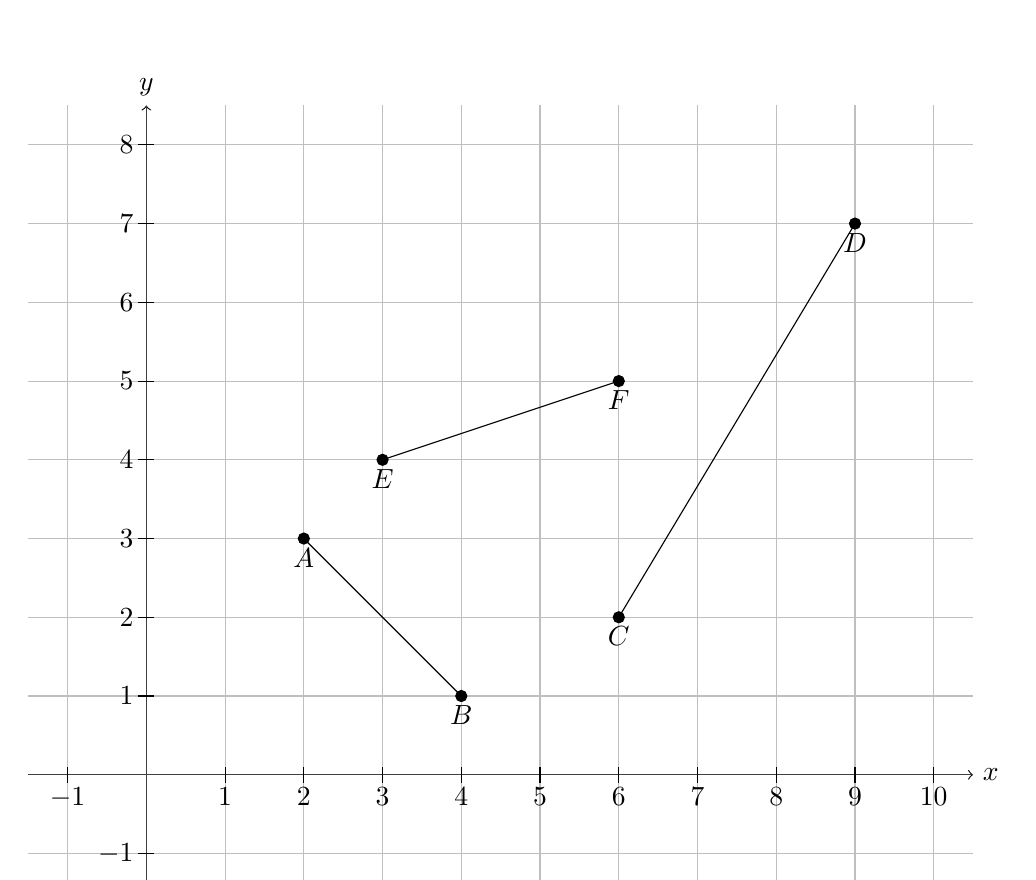
\begin{tikzpicture}
    % Define the axes with labels and numerical ticks
    \draw[->] (-1.5,0) -- (10.5,0) node[right] {$x$}; % X-axis with label
    \draw[->] (0,-1.5) -- (0,8.5) node[above] {$y$}; % Y-axis with label
    
    % Add translucent grid lines (using opacity)
    \draw[gray, opacity=0.5] (-1.5,-1.5) grid (10.5,8.5);
    
    % Add numerical labels along the axes
    \foreach \x in {-1,1,2,3,4,5,6,7,8,9,10}
        \draw (\x,-0.1) -- (\x,0.1) node[below=4pt] {$\x$};
    \foreach \y in {-1,1,2,3,4,5,6,7,8}
        \draw (-0.1,\y) -- (0.1,\y) node[left=4pt] {$\y$};
    
    % Add labels to some points
    \filldraw (2,3) circle (2pt) node[below] {$A$};
    \filldraw (4,1) circle (2pt) node[below] {$B$};
    \filldraw (6,2) circle (2pt) node[below] {$C$};
    \filldraw (9,7) circle (2pt) node[below] {$D$};
    \filldraw (3,4) circle (2pt) node[below] {$E$};
    \filldraw (6,5) circle (2pt) node[below] {$F$};

    % Draw a line segment from A to B
    \draw[black] (2,3) -- (4,1);
    \draw[black] (6,2) -- (9,7);
    \draw[black] (3,4) -- (6,5);
    
\end{tikzpicture}

\newpage

\section*{Task 3}

\begin{enumerate}
    \item (2,4) \& (3,5)
    \begin{align*}
        d_{cd} &= |3-2|+|5-4|\\
        &=|1|+|1|\\
        &=2\\ 
    \end{align*}
    \item (2,4) \& (5,3)
    \begin{align*}
        d_{cd} &= |5-2|+|3-4|\\
        &=|3|+|-1|\\
        &=4\\ 
    \end{align*}
    \item (2,4) \& (7,1)
    \begin{align*}
        d_{cd} &= |7-2|+|1-4|\\
        &=|5|+|-3|\\
        &=8\\ 
    \end{align*}
    \item (2,4) \& (6,8)
    \begin{align*}
        d_{cd} &= |6-2|+|8-4|\\
        &=|4|+|4|\\
        &=8\\ 
    \end{align*}
\end{enumerate}

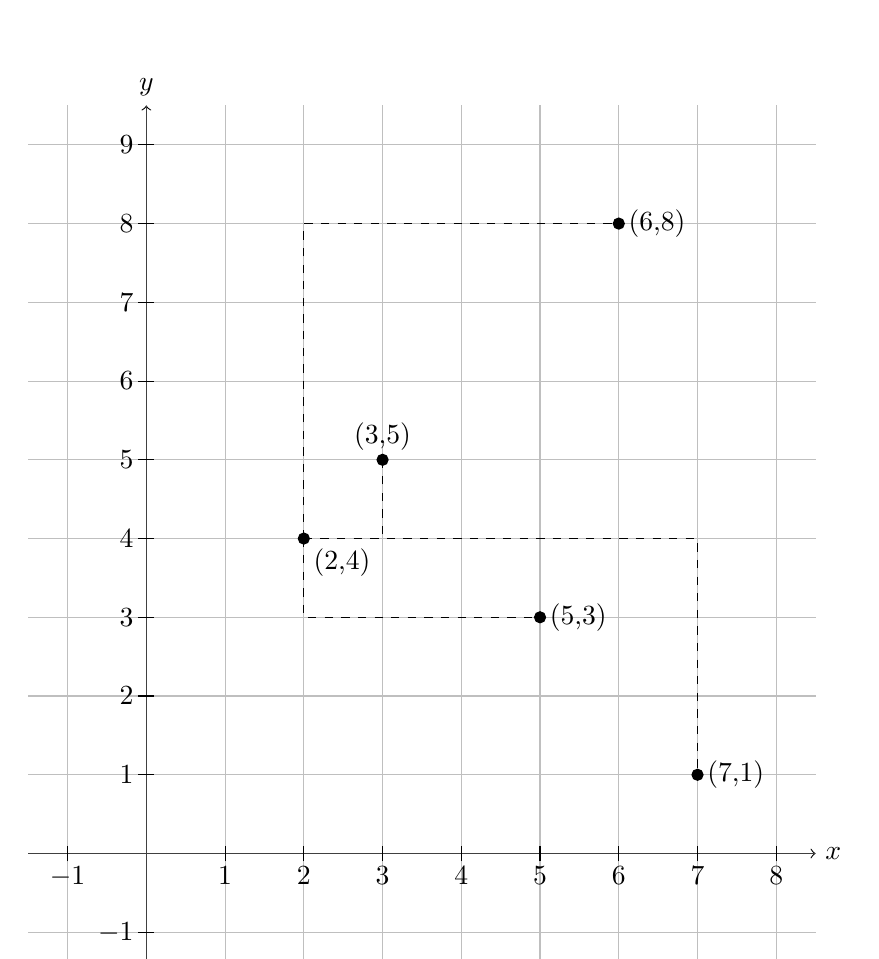
\begin{tikzpicture}
    % Define the axes with labels and numerical ticks
    \draw[->] (-1.5,0) -- (8.5,0) node[right] {$x$}; % X-axis with label
    \draw[->] (0,-1.5) -- (0,9.5) node[above] {$y$}; % Y-axis with label
    
    % Add translucent grid lines (using opacity)
    \draw[gray, opacity=0.5] (-1.5,-1.5) grid (8.5,9.5);
    
    % Add numerical labels along the axes
    \foreach \x in {-1,1,2,3,4,5,6,7,8}
        \draw (\x,-0.1) -- (\x,0.1) node[below=4pt] {$\x$};
    \foreach \y in {-1,1,2,3,4,5,6,7,8,9}
        \draw (-0.1,\y) -- (0.1,\y) node[left=4pt] {$\y$};
    
    % Add labels to some points
    \filldraw (2,4) circle (2pt) node[below right] {(2,4)};
    \filldraw (3,5) circle (2pt) node[above] {(3,5)};
    \filldraw (5,3) circle (2pt) node[right] {(5,3)};
    \filldraw (7,1) circle (2pt) node[right] {(7,1)};
    \filldraw (6,8) circle (2pt) node[right] {(6,8)};
    
    % Draw a line segment representing Manhattan distance
    \draw[black, dashed] (2,4) -- (3,4) -- (3,5);
    \draw[black, dashed] (2,4) -- (2,3) -- (5,3);
    \draw[black, dashed] (2,4) -- (7,4) -- (7,1);
    \draw[black, dashed] (2,4) -- (2,8) -- (6,8);
    
\end{tikzpicture}

\newpage

\section*{Task 4}

\includegraphics[width=0.95\textwidth]{images/figures/fig2.png}

\newpage

\section*{Task 5}

The Euclidean and City Block distance is method of measuring difference between two point to get the distance betweeen the two point. The Euclidean distance measure the shortest distance in a straight line, while the City Block measure the absolute distance betweeen two point from every axis or dimension it has.

The Euclidean formula goes as followed:
\begin{center}
    $d=\sqrt{(x_2-x_1)^2+(y_2-y_1)^2+(z_2-z_1)^2}$
\end{center}
Adding more Variables as the dimension increase or for n-dimension it can be rewritten as 
\begin{center}
    $d=\sqrt{\sum_{i=1}^{k}(p_i-q_i)}$
\end{center}
While the City Block formula goes as followed: 
\begin{center}
    $d_{cd}=|x_2-x_1|+|y_2-y_1|+|z_2-z_1|$
\end{center}
Adding more Variables as the dimension increase or for n-dimension it can be rewritten as
\begin{center}
    $d_{cd}=\sum_{i=1}^{k}|p_i-q_i|$
\end{center}

An applicative example of both method of measurement is for measuring shortest distance betweeen two point. Other use of both method including but not limited to calculating the distance between two rows of data, clustering, and etc.

\end{document}